
\section{Implementation}
In this section we will present WAZIUP platform components and the technology and tools selected for each component.

\subsection{Platform components}
Here is a detailed view of WAZIUP platform components:

\begin{figure}[h!]
\centering
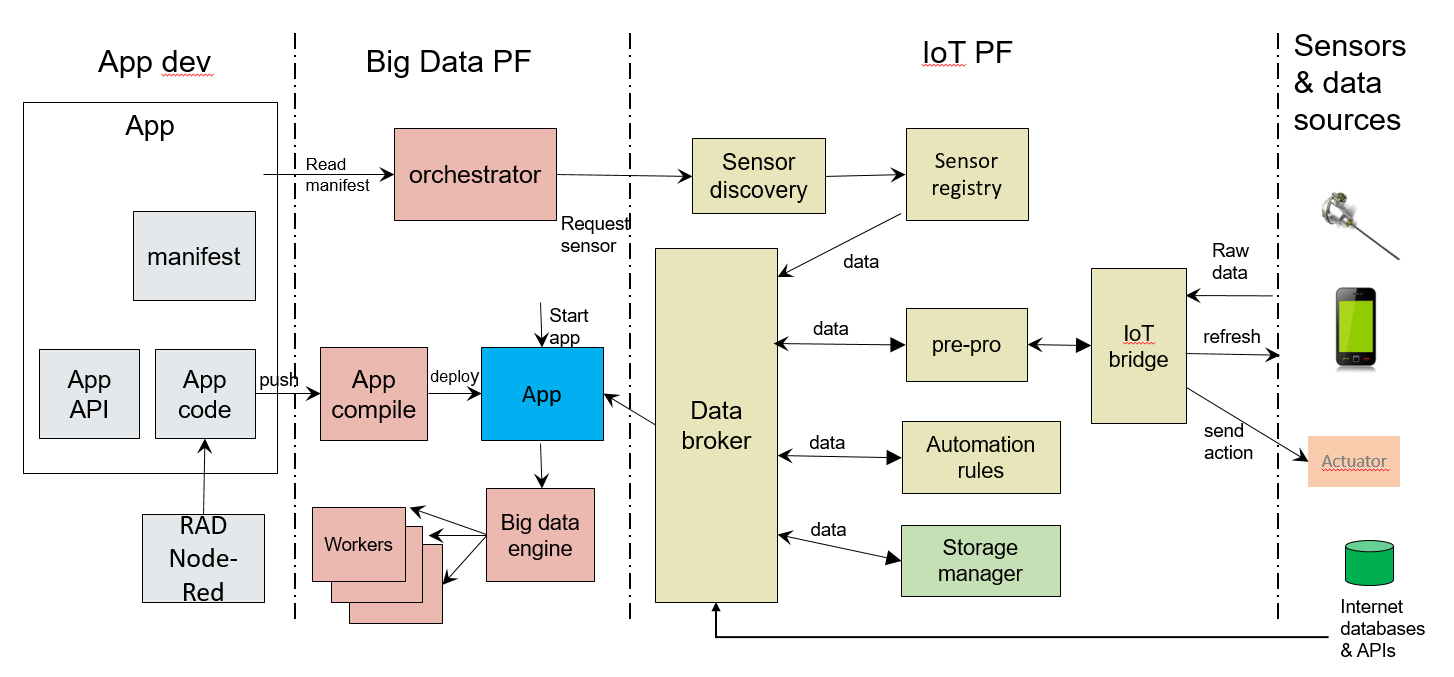
\includegraphics[width=0.9\textwidth]{figs/platformOverview.png}
\caption{WAZIUP IoT platform overview}
\label{fig:platformOverview}
\end{figure}

The figure ~\ref{fig:platformOverview} presents the full WAZIUP architecture. 
There are 4 silos (from left to right): Application development, big data platform, IoT platform, Sensors and data sources. 
The first silo involves the development of the application itself. 
A rapid application development (RAD) tool can be used, such as Node-Red. 
The user provides the code source of the application, together with the manifest. 
The manifest describes the requirements of the application in terms of:
\begin{itemize}
	\item \emph{Compute needs (i.e RAM, CPU, disk)}
	\item \emph{reference to data sources (i.e. sensors, internet - sources...)}
	\item \emph{big data engines needed (i.e Flink, Hadoop...)}
	\item \emph{configuration of sensors (i.e. sampling rate)}
	\item \emph{local and global application deployment}
\end{itemize}

The application source code, together with the manifest, is pushed to the Waziup Cloud platform by the user. 
The orchestrator component will read the manifest and trigger the compilation of the application. 
It will then deploy the application in the Cloud execution environment. 
It will also instantiate the services needed by the application, as described in the manifest. 
The last task of the orchestrator is to request the sensor and data sources connections from the IoT components of the architecture. 
The sensor discovery module will be in charge of retrieving a list of sensors that matches the manifest description.
On the left side of the diagram, the sensor owners can register their sensors with the platform. 
External data sources such as Internet APIs can also be connected directly to the data broker. 
The sensors selected for each application will deliver their data to the data broker, through the IoT bridge and preprocessor. 
The IoT bridge is responsible on the senors communication, it receives and transmits data to sensors using its specific protocol. 
The pre-process can apply transformation of the received data. 
Since internet connectivity is intermittenet, local storage and local automated rules are need. 
The automation rules component is responsible on executing local predefined rules and the storage manager is responsible on storing historic data.

\subsection{Sequence diagrams}
In this section the main two more important sequence diagrams are presented. 

\begin{figure}[h!]
\centering
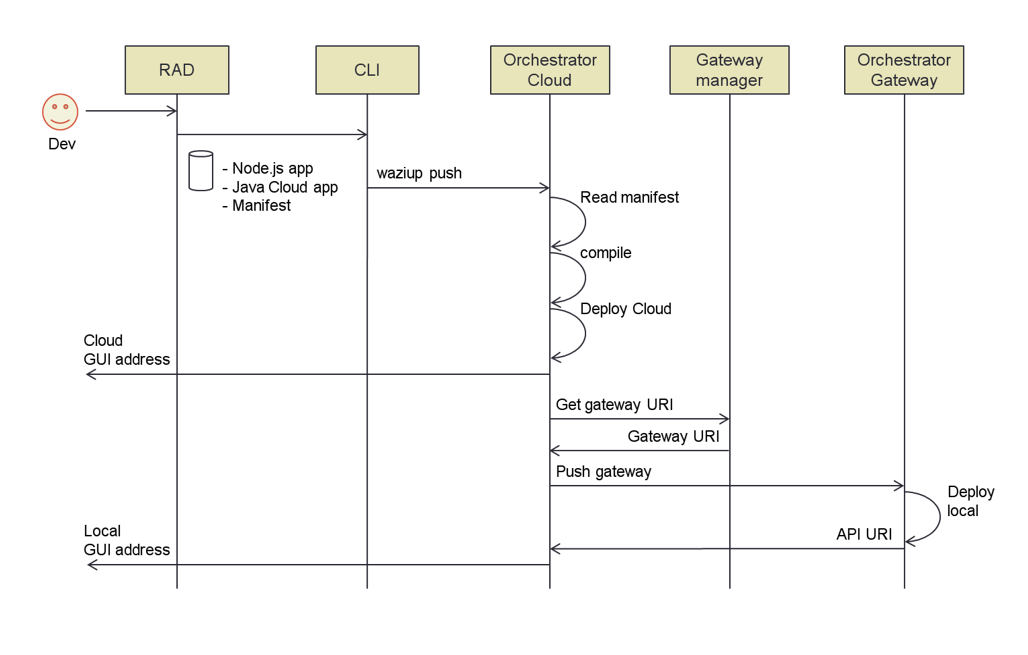
\includegraphics[width=0.9\textwidth]{figs/SeqdeployApp.png}
\caption{Application deployment sequence diagram}
\label{fig:SeqdeployApp}
\end{figure}

The Figure ~\ref{fig:SeqdeployApp} shows the sequence of an application deployment on Waziup platform. First, the developer uses the RAD to create a program source code. It is then pushed on Waziup platform using Waziup CLI. The Orchestrator of the Cloud instance read the manifest, compiles the application and deploys it in the Cloud execution environment. Using the information from the manifest and the gateway manager, it will also select the gateways where the application needs to be deployed. It will then contact the orchestrator from the corresponding gateways and ask them to deploy the application. If the gateway is not available at the moment, this action is delayed.

\begin{figure}[h!]
\centering
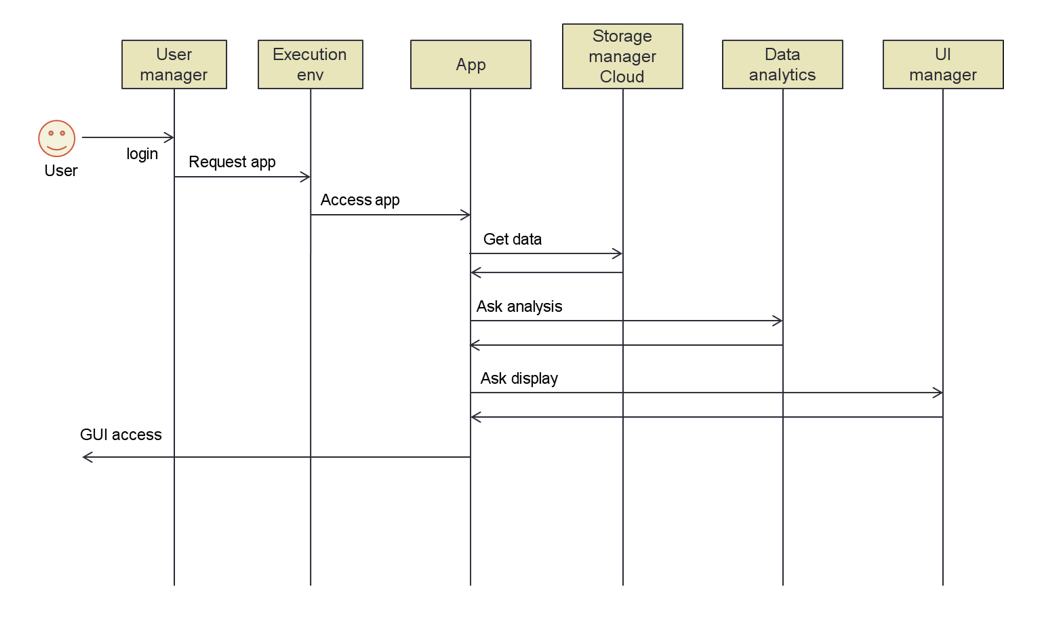
\includegraphics[width=0.9\textwidth]{figs/seqRunApp.png}
\caption{Application run sequence diagram}
\label{fig:seqRunApp}
\end{figure}

The Figure ~\ref{fig:seqRunApp} shows the sequence followed by a running application. First of all a user request the access to an application to the user manager, using his login and password. If granted, the User manager will forward the request to the execution environment which gives access to the app. The app is then getting its data from the Cloud Storage manager. It is further pushing the data to the data analytics component in order to get the elaboration. This elaborated data is then sent to the UI manager, in order to be displayed to the user.

\subsection{Technology and tools}

In this section the technology choices for each functional component stated above will be presented.
\paragraph{ In the cloud level,} functional components are the data broker, data registry and data discovery.
To cover these functionalities, The FIWARE generic enabler Orion context broker is the all-in-one solution.
It is based on the Next Generic Service Interfaces (NGSI) 9/10.
NGSI specification defines a data model and interfaces to manage the whole cycle of virtual entities.  
other components can also be an option : the Nec IoT broker that covers the functionality of the data broker and uses the ConfMan component for the data discovery and registry.

\paragraph{In the gateway level,} these functionalities have been identified:

\begin{itemize}
    \item \emph{Multiprotocol}
The FIWARE IoT agent component: can be an option to ensure this characteristic. 
Each IoT agent can be responsible on the data transfer to and from the devices using the device specific protocol. 
    \item \emph{Device management}
The LwM2M device management protocol is a good candidate, it is a light weight protocol specified by Oma .
    \item \emph{Automation rules}
FIWARE Cepheus enabler can be an option since it has a complex event processing engine. 
    \item \emph{Data processing}
this component will be developed depending on use cases requirements.
    \item \emph{Data storage}
Mongo DB can be an option, other light data bases can be also considered such as SQLiteDB.
\end{itemize}

\paragraph{In the devices and networking level,} LoRa technology captured our attention. 
It specifies LoRaWAN for Low Power Wide Area Network (LPWAN), the kind of technology needed in our project context (rural environment). 
Using LoRaWAN we can reach above 20 km in Line-Of-Sight (LOS) condition between devices and the gateway. 

